%Template for ICIP-2014 paper; to be used with:
%          spconf.sty  - ICASSP/ICIP LaTeX style file, and
%          IEEEbib.bst - IEEE bibliography style file.
% --------------------------------------------------------------------------
\documentclass{article}
\usepackage{spconf,amsmath,graphicx}
\usepackage[ruled, linesnumbered]{algorithm2e}

% Example definitions.
% --------------------
\def\x{{\mathbf x}}
\def\L{{\cal L}}

% Title.
% ------
\title{Robust Vertex Extraction Methods for Convex and Concave Polygons}
% TODO 进行拼写检查
%
% Single address.
% ---------------
\name{Zhou Xiong}
\address{Harbin Institute of Technology\\Computer Science and Engineering\\Harbin, China}

%
% For example:
% ------------
%\address{School\\
%       Department\\
%       Address}
%
% Two addresses (uncomment and modify for two-address case).
% ----------------------------------------------------------
%\twoauthors
%  {A. Author-one, B. Author-two\sthanks{Thanks to XYZ agency for funding.}}
%       {School A-B\\
%       Department A-B\\
%       Address A-B}
%  {C. Author-three, D. Author-four\sthanks{The fourth author performed the work
%       while at ...}}
%       {School C-D\\
%       Department C-D\\
%       Address C-D}
%
\begin{document}
%\ninept
%
\maketitle
%
\begin{abstract}

Locating the vertices of a polygonal digital contour is an important but seldom addressed problem.
We propose two fast and robust methods for vertex detection in convex and non-convex polygons.
The first method is dedicated to convex polygons. We first map each point to the unit circle, then apply
k-means to assign points the corresponding lines, vertices are computed as the intersection of adjacent lines.
The mapping in the method can preserve the topological order of points, which is a key contribution of our method.
The second method does not require the polygon to be convex. We use the RANSAC approach to fit the polygon. A polygon
is modeled as consecutive lines, we iterate several times and choose the model with highest inliner rate. 
Experiments on natural and synthetical images are given to show the validity of our approach.

\end{abstract}
%
\begin{keywords}
  Vertex detection, Convex Hull, K-means, RANSAC
\end{keywords}
%
\section{Introduction}
\label{sec:intro}
%The work on the detection of dominant points started from the research of Attneave who proposed that the local maximum
%curvature points on a curve have a rich information content and are sufficient to characterize this curve have a rich
%rich information content and are sufficient to characterize this curve. A method for detection of
%dominant points can lead to a good representation of a planar shape at different resolutions.

%In addition, a representation of a planar shape based on dominant points has some advantages.
%Firstly, it enables a high data reduction.
%Secondly, this representation concentrates on principal features of the shape, so it is
%efficient for shape matching, feature extraction or decomposition of curve into meaningful parts.
%Therefore, these points have a critical role in curve approximation, shape matching and image matching.
%They also lead to some applications in other domains of machine vision such as vector data compression.

%Starting from Attneave's work, there are many existing methods for dominant points detection.
%Concerning this problem, several problems in this topic have been identified: evaluation, number of
%parameters, selection of starting point, multi-scale, working with noisy curves, \dots.

%In general, we can classify these methods into two groups.
%The first one contains direct methods that determine dominant points such as high curvature
%value points by using curvature-based significant measures, or using alternative significant
%measures such as k-cosine, region of support (ROS). Rosenfield and Johnston used cosine of the
%angle between the archs of length k on each side of a point (termed k-cosine) as curvature-based
%significant measure.
%The indirect methods are often based on polygonal approximation of the curve,
%the dominant points are deduced after doing this step.
%In these methods, the dominant points are detected as the vertex of approximated polygons.
%In addition, we can divide polygonal approximation methods into three principal approaches:
%sequential approach, split and merge approach, heuristic search one.
%For sequential approach, Ray and Ray determined the longest possible line segment
%with minimum error. Kolesnikov proposed a sub-optimal algorithm for polygon
%approximation of closed curves based on the corresponding optimal dynamic programming
%algorithm for open curves.
%Aoyama used a linear scan to evaluate error conditions, if the conditions are not satisfied,
%a new segment search is started. The problem of this method is that sometimes the nodes
%do not correspond to the corners because a new vector is defined only when the conditions
%are violated.
%For split-and-merge methods, lines are fitted to an initial segmentation of the boundary
%and then the least square error is computed. These methods then iteratively split
%a line if the error is too large and merge two points if the error is too small.
%Heuristic approach is used to reduce the complexity of an optimal algorithm for approximating
%polygon. Genetic algorithm, tabu search, ant colony search, fuzzy ressning are some
%popular techniques approach is simple and fast, but the quality of its result depends on the
%starting point.
%Masood has proposed an efficient method that does not belong to any of the above groups.
%It is based on break point extraction. A break point is a point of which the chain code
%is different from that of the previous point. Break points are taken as initial set of
%dominant points. Each break point are taken as initial set of dominant points.

\subsection{Hough Transform}
\label{sub:Hough Transform}

\subsection{Previous Methods}
\label{sub:Previous Methods}

\subsection{Critical Point}
\label{sub:Critical Point}

\subsection{Polygonal Approximation}
\label{sub:polygon}

\subsection{Computational Geometry}
\label{sub:Computational Geometry}

\subsection{My Method}
\label{sub:My Method}

We adopt ideas from data clustering and machine vision

\section{The method}
\label{sec:The method}

Given a closed curve of a polygon, we want to get the coordinates of its vertices.
Beside the efficiency and simplicity, a practical algorithm must be able
to deal with noisy curves. The vertices of a noisy polygon is a subset of its critical points.
%% 写这里还需要看看Polygonal Approximation的文章,也就是Critical Point的Indirect方法。
Previous methods for critical point detection are mainly local methods. But because the vertex of a
polygon is not a local feature, local method without global post-processing can easily fail on noisy curves.
The two algorithms prosed in this paper are both global methods. They only take the number of vertices
as parameter and are robust to noise and outliers in the curve.

In this section we will introduce two algorithms for extracting the vertices of polygon.
The first algorithm is only viable for convex polygon. Besides its efficiency and robustness,
this algorithm also gives some theoretical insight into the problem of finding vertices on a convex hull.

The second algorithm can deal with general polygon.
The algorithm is a direct application of the RANSAC scheme and thus a iterative algorithm.
By randomly fitting a polygon with lines iteratively, an optimal combination of lines is selected
as the model for the polygon. This algorithm is less efficient than the first algorithm for convex polygons,
but it can extract the vertex of concave polygon, which is a challenging task.


\subsection{The contour}
\label{sub:The contour}

Before introducing the algorithms, we will first describe possible types of input.
We use $\mathbf{C}$ to denote the input contour. $\mathbf{C}$ can be
should consist of consecutive pixels in the sense of 8-way connection. % 看看概念,凭印象写的的

The main procedure of our algorithm is shown in Algorithm~\ref{algo_convex_polygon}.
The proposed method is a global method, all points are taken into consideration at once.

\subsection{Vertex Extraction for Convex Polygon}
\label{sec:Vertex Extraction for Convex Polygon}


\subsection{Vertex Extraction for General Polygon}
\label{sec:Vertex Extraction for General Polygon}


\begin{algorithm}[h]  % h是什么意思?以前查过,现在忘了
  \small              % small不知是什么意思
  \SetKwFunction{FindConvexHull}{FindConvexHull}
  \SetKwFunction{Kmeans}{K-Means-Clustering}
  \SetKwInOut{Input}{Input}
  \SetKwInOut{Output}{Output}
  \SetKwInOut{Task}{Task}
  \Task{Extract vertices of a convex polygonal contour}
  \Input{The contour $\mathbf{C}$, number of vertices $n$}
  \Output{Coordinates of $n$ vertices}
  \BlankLine
  $hull \leftarrow$  \FindConvexHull{$\mathbf{C}$} \;
  $l \leftarrow$  number of points in $hull$ \;
  $vectors \leftarrow $  empty list \;
  \For{$i\leftarrow 1$ \KwTo $l$}{
    \tcp*[h]{compute direction vector} \;
    $v \leftarrow \mathbf{C}[(i+1)\mod l] - \mathbf{C}[i] $  \;
    \tcp*[h]{normalize to unit vector} \;
    $v \leftarrow$   $v$ $/$ $\Vert$ $v$ $\Vert$ \;
    $vectors$.add(v) \;
  }
  $indexes \leftarrow$ \Kmeans{$vectors$, $n$} \;
  Seperate points in $hull$ into $n$ sets by $indexes$  \;
  $lines \leftarrow$ fit the points in each set to a line \;
  $vertices \leftarrow$ the intersection of adjacent lines \;
  \Return $vertices$
  \caption{Vertex Extraction for Convex Polygon}
  \label{algo_convex_polygon}
\end{algorithm}

\begin{algorithm}[h]
  \small
  \SetKwInOut{Input}{Input}
  \SetKwInOut{Output}{Output}
  \SetKwInOut{Task}{Task}
  \SetKwFunction{FitModel}{Fit-Model}
  \Task{Extract vertices of a general polygonal contour}
  \Input{The contour $\mathbf{C}$, number of vertices $n$}
  \Output{Coordinates of $n$ vertices}
  \BlankLine
  $inlinerRate \leftarrow -1$ \;
  $lines \leftarrow$ empty list \;
  $N \leftarrow 100 $\; % number of trial
  $d \leftarrow 2.5 $\; % error
  \tcp*[h]{main procedure of RANSAC} \;
  \For{$i\leftarrow 1$ \KwTo $N$}{
    \tcp*[h]{one pass for model fitting} \;
    $linesNew, inlinerRateNew \leftarrow$ \FitModel{ $\mathbf{C}$, $n$, $d$ }\;
    \If{$inlinerRateNew > inlinerRate$} {
      $inlinerRate \leftarrow inlinerRateNew$ \;
      $lines \leftarrow linesNew$ \;
    }
  }
  $lines \leftarrow$ fit the points in each set to a line \;
  $vertices \leftarrow$ the intersection of adjacent lines \;
  \Return $vertices$
  \caption{Vertex Extraction for General Polygon} \label{algo_nonconvex_polygon}
\end{algorithm}

\begin{algorithm}[h]
  \small
  \SetKwInOut{Input}{Input}
  \SetKwInOut{Output}{Output}
  \SetKwInOut{Task}{Task}
  \Task{Fit contour with lines}
  \Input{The contour $\mathbf{C}$, number of lines $n$, error bound $d$}
  \Output{$n$ lines}
  $k \leftarrow $ number of points in $\mathbf{C}$ \;
  $index \leftarrow $ initialize to array of size $k$ \;
  \tcp*[h]{-1 means ``not assigned to line''} \;
  Set all elements in $index$ to -1 \;
  \For{$i\leftarrow 1$ \KwTo $n$}{
    $p \leftarrow$ randomly choose an integer in [1, k] \;
    $line \leftarrow$ fit a line around the $p$th unassigned point \;
    Mark points, in $index$, whose distance from $line$ is smaller than $d$ \;
    $k \leftarrow $ number of -1 in $index$ \;
  }
  $lines \leftarrow$ fit lines according to the mark in $index$ \;
  \Return $lines$ \;
  \caption{Fit a general polygon with lines}\label{fit_model}
\end{algorithm}


% Below is an example of how to insert images. Delete the ``\vspace'' line,
% uncomment the preceding line ``\centerline...'' and replace ``imageX.ps''
% with a suitable PostScript file name.
% -------------------------------------------------------------------------
%\begin{figure}[t]

%\begin{minipage}[b]{1.0\linewidth}
  %\centering
  %\centerline{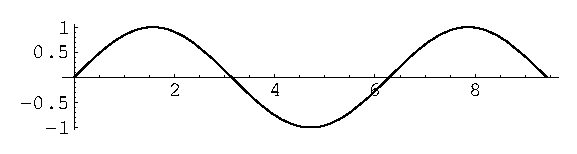
\includegraphics[width=8.5cm]{Figures/image1}}
%%  \vspace{2.0cm}
  %\centerline{(a) Result 1}\medskip
%\end{minipage}
%%
%\begin{minipage}[b]{.48\linewidth}
  %\centering
  %\centerline{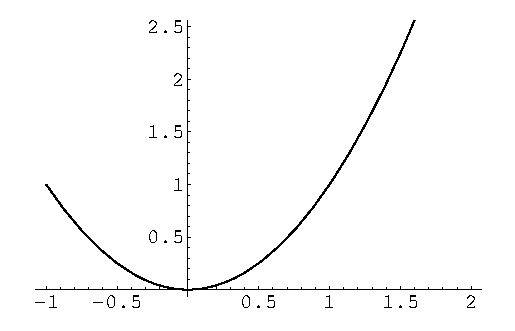
\includegraphics[width=4.0cm]{Figures/image3}}
%%  \vspace{1.5cm}
  %\centerline{(b) Results 3}\medskip
%\end{minipage}
%\hfill
%\begin{minipage}[b]{0.48\linewidth}
  %\centering
  %\centerline{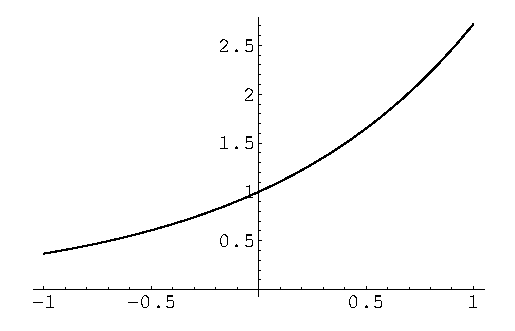
\includegraphics[width=4.0cm]{Figures/image4}}
%%  \vspace{1.5cm}
  %\centerline{(c) Result 4}\medskip
%\end{minipage}
%%
%\caption{Example of placing a figure with experimental results.}
%\label{fig:res}
%%
%\end{figure}


\section{Experiments}
\label{sec:Experiments}


% To start a new column (but not a new page) and help balance the last-page
% column length use \vfill\pagebreak.
% -------------------------------------------------------------------------
%\vfill
%\pagebreak

\section{Conclusion}
\label{sec:Conclusion}


% References should be produced using the bibtex program from suitable
% BiBTeX files (here: refs). The IEEEbib.bst bibliography
% style file from IEEE produces unsorted bibliography list.
% -------------------------------------------------------------------------
\bibliographystyle{IEEEbib}
\nocite{*}

\bibliography{refs}

\end{document}
